\documentclass[11pt,a4paper,twoside,openright]{report}

\usepackage[pdftex]{graphicx} % Biblioteca para uso de figuras
\usepackage{color}

\usepackage[brazil]{babel} % Biblioteca para uso da l�ngua portuguesa
\usepackage[T1]{fontenc} % Biblioteca para uso da acentua��o de entrada
\usepackage[latin1]{inputenc} % Biblioteca para uso da acentua��o de sa�da

\usepackage{amsthm,amsfonts,amsmath,amssymb}  % Biblioteca para uso de comandos matem�ticos
\usepackage{pslatex}
\usepackage{pstricks,pst-node,color,pst-gantt,pst-coil}
\usepackage{scalefnt}
\usepackage{float} %Permite colocar "\begin{figure}[H]" e colocar imagem exatamente onde desejar
\usepackage[hyphens]{url} % Para Aceitar URL nas referencias
\usepackage{pdfpages}

\usepackage{eurosym} %Pacote para possibilitar o uso do s�mbolo de euro "\euro"

\usepackage{listings} % para importa��o de c�digos fonte 

\usepackage{comment}
\usepackage[margin=2.7cm]{geometry}
\renewcommand{\baselinestretch}{1.5}

\setlength{\parskip}{0em}

% Pacote para configurar cabe�alho e rodap�
\usepackage{fancyhdr}
\pagestyle{empty}
\fancyhf{} % clear all header and footer fields

\fancypagestyle{plain}{\pagestyle{fancy}}
\renewcommand{\headrulewidth}{0pt}
\renewcommand{\footrulewidth}{0pt}

%Pacote para organizar apendices 
\usepackage[titletoc]{appendix}

%%%%%%%%%%%%%%%%%%%%%%%%%%%%%%%%%%%%%% CONFIGURA��ES DE ANEXOS %%%%%%%%%%%%%%%%%%%%%%%%%%%%%%%%%%%%%%

\newcommand{\annexname}{Anexo}
\makeatletter
\newcommand\annex{\par
  \setcounter{chapter}{0}%
  \setcounter{section}{0}%
  \gdef\@chapapp{\annexname}%
  \gdef\thechapter{\@Roman\c@chapter}}
\makeatother

\newenvironment{poliabstract}[1]
  {\renewcommand{\abstractname}{#1}\begin{abstract}}
  {\end{abstract}}

%%%%%%%%%%%%%%%%%%%%%%%%%%%%%%%%%%%%%% CONFIGURA��ES DE P�GINA %%%%%%%%%%%%%%%%%%%%%%%%%%%%%%%%%%%%%%
%\topmargin -2.1cm
%\oddsidemargin 0.5cm 
%\evensidemargin 0.5cm 
%\textwidth 15cm
%\textheight 25.1cm
	
%%%%%%%%%%%%%%%%%%%%%%%%%%%%%%%%%%%%%%%% IN�CIO DO DOCUMENTO %%%%%%%%%%%%%%%%%%%%%%%%%%%%%%%%%%%%%%%%
\begin{document}
	
%%%%%%%%%%%%%%%%%%%%%%%%%%%%%%%%%%%%%%  INCLUDES %%%%%%%%%%%%%%%%%%%%%%%%%%%%%%%%%%%%%%

%%%%%%%%%%%%%%%%%%%%%%%%%%%%%%%%%%%%%% ELEMENTOS PR�-TEXTUAIS %%%%%%%%%%%%%%%%%%%%%%%%%%%%%%%%%%%%%%
%%%%%%%%%%%%%%%%%%%%%%%%%%%%%%%%%%%%%%% CONFIGURA??ES DE CAPA %%%%%%%%%%%%%%%%%%%%%%%%%%%%%%%%%%%%%%%
\begin{titlepage}

	% CAPA PRINCIPAL
	\begin{center}
		\Huge{UNIVERSIDADE DE S�O PAULO}\\
		\vspace{0.02\textheight}
		\huge{ESCOLA DE ENGENHARIA DE S�O CARLOS}\\
		\vspace{0.01\textheight}
		\huge{DEPARTAMENTO DE ENGENHARIA EL�TRICA E DE COMPUTA��O}\\
		\vspace{0.2\textheight}
		\huge{\textbf{SEL0630 - Aplica��es de Microprocessadores II}}
		\vspace{0.1\textheight}
		\huge{\textbf{R3V - \emph{Remote 3D Viewer}}}
		\vspace{0.1\textheight}
	\end{center}

		\large
		{
			\begin{flushleft}
			\Large{ \textbf{Autor(es)}:	\hspace{0,2cm} Davi Di�rio Mendes 7546989 \\
																	\hspace{2,55cm} Henrique Alberto Rusa 7593714}\\
			\Large{ \textbf{Professor}: \hspace{0.3cm} Evandro Luis Linhari Rodrigues }\\
			\end{flushleft}

			\begin{center}
				\vspace{0.09\textheight}
				\Large{2015}
			\end{center}
		}

\end{titlepage}


%%%%%%%%%%%%%%%%%%%%%%%%%%%%%%%%%%%%%%%%%%%%%%% INSER??O P?GINA EM BRANCO %%%%%%%%%%%%%%%%%%%%%%%%%%%%%%%%%%%%%%%%%%%%%%
\cleardoublepage


%%%%%%%%%%%%%%%%%%%%%%%%%%%%%%%%%%%%%%%%%%%%%%% RESUMO - PORTUGUES %%%%%%%%%%%%%%%%%%%%%%%%%%%%%%%%%%%%%%%%%%%%%%
\
\vspace{0.11\textheight}

\begin{center}
\textbf{\Huge{Resumo}}
\end{center}

\vspace{0.05\textheight}

Texto em um par�grafo apenas - deve conter "tudo" resumidamente (introdu��o, m�todo(s), resultados e conclus�es), de tal forma que seja poss�vel compreender a proposta e o que foi alcan�ado.

\vspace{0.05\textheight}

Palavras-Chave: palavra1, palavra2, palavra3, palavra4, palavra5.

%%%%%%%%%%%%%%%%%%%%%%%%%%%%%%%%%%%%%%%%%%%%%%% INSER??O P?GINA EM BRANCO %%%%%%%%%%%%%%%%%%%%%%%%%%%%%%%%%%%%%%%%%%%%%%
\cleardoublepage



%%%%%%%%%%%%%%%%%%%%%%%%%%%%%%%%%%%%% CONFIGURA��ES DOS �NDICES %%%%%%%%%%%%%%%%%%%%%%%%%%%%%%%%%%%%%
%\usepackage{fancyhdr}
\pagestyle{fancy}
\fancyhf{} % clear all header and footer fields
\fancyhead[RO, LE] {\thepage}

\fancypagestyle{plain}{\pagestyle{fancy}}

\tableofcontents % �ndice Geral


%%%%%%%%%%%%%%%%%%%%%%%%%%%%%%%%%%%%%%%% ADI��O DOS CAP�TULOS %%%%%%%%%%%%%%%%%%%%%%%%%%%%%%%%%%%%%%%	
\chapter{Introdu��o}
\label{Introducao}

\hspace{0,5cm}
Realmente introduz o leitor indicando quais s�o as dire��es do trabalho ? apresenta o tema e o objeto do trabalho e cont�m as Refer�ncias do Estado da arte (quem est� fazendo e em que n�vel os trabalhos da �rea est�o hoje) \cite{referencia1}.

Outra refer�ncia para a bibliografia \cite{referencia2}.

Segundo \cite{referencia3} h� uma sequ�ncia l�gica para a reda��o da monografia como apresenta em \cite{enzo}.

Refer�ncia para a figura \ref{logo}.

\begin{figure}[H]
 	\centering
 	
\includegraphics[scale=0.35]{./Resources/logo_eesc_vertical.png}
 	\caption{Logo da EESC.}
 	\label{logo}
 \end{figure}



% % % % % % % % % % % % % % % % % % % % % % % % % % % % % % % % % % % % % % % % % % % % % % % % % % %
\section{Objetivos}
\hspace{0,5cm}
Objetivos do trabalho.



% % % % % % % % % % % % % % % % % % % % % % % % % % % % % % % % % % % % % % % % % % % % % % % % % % %
\section{Motiva��o (opcional)}
\hspace{0,5cm}
Descrever a motiva��o do trabalho.


% % % % % % % % % % % % % % % % % % % % % % % % % % % % % % % % % % % % % % % % % % % % % % % % % % %
\section {Justificativas/relev�ncia(opcional)}
\hspace{0,5cm}
Justificativa do trabalho.


% % % % % % % % % % % % % % % % % % % % % % % % % % % % % % % % % % % % % % % % % % % % % % % % % % %
\section {Organiza��o do Trabalho(opcional)}
\hspace{0,5cm}
Este trabalho est� distribu�do em XXX cap�tulos, incluindo esta introdu��o, dispostos conforme a descri��o que segue:

Cap�tulo 2: Descreve .....................................................................................

Cap�tulo 3: Discorre sobre .....................................................................................

Cap�tulo 4: Apresenta .....................................................................................




























\chapter{Embasamento Te�rico}
\label{EmbasamentoTeorico}
\hspace{0,5cm}

  Na fase de projeto do sistema R3V proposto foram elencados conhecimentos e fundamentos necess�rios para o desenvolvimento do mesmo. Com isso em mente, pode-se discursar melhor sobre os t�picos mais relevantes do sistema, permitindo que o leitor aprofunde-se devidamente para que, ao final, os objetivos do projeto sejam melhor discutidos e compreendidos.

  Neste cap�tulo pretende-se analisar os conceitos de estereoscopia, sistemas embarcados, sistemas distribu�dos e \emph{dead reckoning}.

      % Revis�o da literatura dos t�picos  que sustentam a ci�ncia e o conhecimento, relativos aos objetivos e aos m�todos escolhidos para o desenvolvimento do trabalho.

      % Itens como Considera��es Iniciais e Finais n�o s�o obrigat�rios, mas completam muito bem qualquer cap�tulo.


  \section{Estereoscopia} % rebs

    A simula��o de imagens em tr�s dimens�es (vis�o espacial) � associada ao conceito da estereoscopia. Para isso, o c�rebro humano necessita adiquirir duas imagens, cada qual com um leve deslocamento lateral (angular), e com estas calcular a profundidade dos objetos \cite{esteves2011estereoscopia} \cite{momm2001prototipo}.

    Existem tamb�m t�cnicas de percep��o do espa�o tri-dimensional que avaliam sombras, sobreposi��o de objetos numa cena e v�rios outros par�metros, possibilitando verificar a disposi��o dos elementos no espa�o.

    Entretanto, existe uma diferen�a fundamental entre percep��o e simula��o do espa�o tri-dimensioanl para o usu�rio, apresentadas a seguir.

    \begin{itemize}
      \item \textbf{Percep��o Tri-dimensonal:} O usu�rio consegue perceber a disposi��o dos elementos numa imagem (profundidade relativa, dist�ncia relativa entre objetos) somente a partir da an�lise de uma imagem que possui indicativos como sombra, ilumina��o e outros.
      \item \textbf{Simula��o Tri-dimensonal:} O usu�rio tem a sensa��o de que os objetos possuem dimens�es reais, com tamanho e profundidade bem definidos; a dist�ncia entre elementos � percebida, entretanto n�o mais pela sombra, mas pela pr�pria proje��o da simula��o em si.
    \end{itemize}

    Portanto, enquanto o usu�rio pode perceber a terceira dimens�o em valores relativos (objetos mais pr�ximos ou mais afastados, maiores ou menores), a simula��o do espa�o tri-dimensioanl � realizada pela sobreposi��o de imagens com mesmo ponto focal mas deslocadas levemente uma da outra, possibilitando a reconstru��o, pelo c�rebro, da profundidade dos elementos.

  \section{Sistemas Embarcados}

    Segundo White (2011, p.1) a defini��o de sistemas embarcados varia de
    pessoas para pessoas. Para algu�m acostumado a lidar com servidores,
    programa��o para dispositivos m�veis pode ser considerada como um
    desenvolvimento embarcado. Por outro lado, para aquele acostumado a
    trabalhar com microcontroladores de 8-bits, qualquer coisa com um sistema
    operacional n�o parece muito embarcado. Mas ela enuncia a defini��o: ``um
    sistema embarcado � um sistema computadorizado constru�do propositadamente
    para sua aplica��o'' \cite{White:2011:MES:2161614}.

    Desta forma podemos real�ar a diferen�a entre sistemas computacionais e
    sistemas embarcados. Enquanto sistemas computacionas s�o desenvolvidos para
    atuar em computadores de prop�sito geral, sistemas embarcados s�o
    desenvolvidos de forma a serem embarcados em \emph{hardware} com prop�sitos
    espec�ficos, visando a aplica��o.

  \section{Sistemas Distribu�dos}

    Sistemas distribu�dos � algo de dif�cil defini��o. Cada autor utiliza uma
    defini��o diferente, embora todas remetam que h� computadores, ou outro
    dispositivo com capacidade de processamento, trabalhando em conjunto.
    Vamos tomar por defini��o: ``Um sistema distribu�do � aquele no qual os
    componentes localizados em computadores interligados em rede se comunicam e
    coordenam suas a��es apenas passando mensagens.'' \cite{coulouris2007sistemas}.

  \section{\emph{WebServices REST}}
    Hoje a internet n�o � mais simplesmente uma ferramenta de difus�o de
    informa��o. Diversos servi�os s�o prestados atrav�s dos \emph{Web Services}.
    Normalmente envolvem um processo burocr�tico rigoroso, como requisi��es
    SOAP ou outros tipos de mensagem, conforme o protocolo seguido. A id�ia de
    um \emph{WebService} REST � de prover servi�os diretamente sobre o
    protocolo HTTP, sem a necessidade de adicionar uma camada de protocolo de
    servi�o \cite{dal2009web}. Servi�os \emph{REST} est�o se popularizando cada vez mais, dada a
    baixa complexidade do sistema e f�cil integra��o por parte dos usu�rios.

  \section{\emph{Dead Reckoning}} % rebs

    A tecnologia prov� diversos sistemas de posicionamento por sensores, \emph{beacons} (refer�ncias fixas no espa�o), equival�ncia entre mapas e outros. Entretanto, pode-se distinguir duas metodologias utilizadas: posicionamento relativo e absoluto \cite{borenstein1994umbmark}.

    \begin{itemize}
      \item \textbf{Absoluto:} Se vale de t�cnicas de sensoreamento com refer�ncias fixas, previamente implementadas, o que adiciona um custo muito alto para cosntru��o e manuten��o destes sistemas espalhados pelo terreno em quest�o.
      \item \textbf{Relativo:} Prop�e uma formula��o mais elegante, se valendo de sensores e par�metros intr�nsecos da implementa��o. Com isso, pode-se estimar a posi��o atual do elemento de acordo com movimenta��es percept�veis ao sistema.
    \end{itemize}

    \emph{Dead reckoning} � uma implementa��o de posicionamento relativo que permite o programador avaliar os diversos sensores para se estimar a localiza��o entre os per�odos de tempos avaliados.

    Note que as duas implementa��es de posicionamento possuem suas vantagens e desvantagens, sendo que uma estimativa de localiza��o (posi��o relativa) adiciona erros �s medidas, enquanto que a outra possui as refer�ncias extremamente precisas (posi��o absoluta).

\section{Rota��o dos Eixos}

  A decomposi��o dos movimentos de rota��o de um usu�rio utilizando um �culos de virtualiza��o � realizada com movimentos angulares, descritas pelos valores \emph{pitch}, \emph{yaw} e \emph{roll}. \\
  A figura \ref{rotacao} apresenta a orienta��o das rota��es descritas anteriormente.

  \begin{figure}[H]
    \centering
    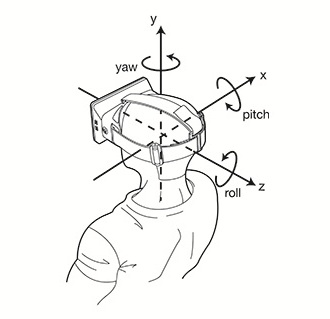
\includegraphics[scale=1.1]{./Resources/oculus_head_model}
    \caption{Representa��o dos movimentos de vis�o de um usu�rio (visto em: https://s3.amazonaws.com/static.oculus.com/website/2013/05/oculus\_head\_model.jpg)}
    \label{rotacao}
   \end{figure}










\chapter{Materiais e M�todos}
\label{Materiais}
\hspace{0,5cm}
Descri��o clara dos procedimentos e dos materiais adotados para o desenvolvimento do trabalho (sem resultados) - incluindo sua adequa��o ao trabalho.

Tem que responder �s perguntas:
-est� com um tamanho adequado (proporcional) � monografia?
-h� informa��o suficiente e clara sobre os materiais e sobre os m�todos  adotados?

N�o h� necessidade de reproduzir (copiar) as obras que embasam o trabalho e sim colocar o suficiente para o entendimento do trabalho e citar as refer�ncias.



% % % % % % % % % % % % % % % % % % % % % % % % % % % % % % % % % % % % % % % % % % % % % % % % % % %
\section{Materiais}
\hspace{0,5cm}
Materiais utilizados no projeto.

  \subsection{Intel Galileo}

  \subsection{Smartphone Android}

  \subsection{IPCam}

  \subsection{Flask}
% % % % % % % % % % % % % % % % % % % % % % % % % % % % % % % % % % % % % % % % % % % % % % % % % % %
\section{M�todos}
\hspace{0,5cm}
M�todos utilizados no projeto.

  \subsection{MJPEG}
  \subsection{\emph{Dead Reckoning}}
  \subsection{Applica��o Cliente}




\chapter{Resultados e Discuss�es}
\label{Resultados}
\hspace{0,5cm}

Aqui se mostra o que o trabalho permitiu produzir, e �s vezes o que pode ser comparado com outros trabalhos - aqui ficam claras se as propostas do trabalho s�o relevantes ou n�o, pois devem permitir a discuss�o do trabalho.

Deve responder: Os resultados est�o claros em bom n�mero (nem muito nem pouco) que permitam avaliar realmente a proposta e o que foi produzido.





\chapter{Conclus�o}
\label{Conclusao}
\hspace{0,5cm}

Durante o desenvolvimento de projeto os objetivos foram alcan�ados com qualidade superior � esperada. O �nico ponto que ficou em falta foi o desenvolvimento do algoritmo de Parallax para estimar imagens 3D baseado em uma �nica imagem 2D.



\section*{Trabalhos futuros}
\hspace{0,5cm}

O prot�tipo se encontra numa fase inicial de desenvolvimento, onde muito pode se fazer para otimizar e aperfei�oar os processos e servi�os utilizados.\\
Com isso, prop�e-se a cria��o de uma c�mera atrelada � placa de desenvolvimento Galileo onde se utilizaria motores mais precisos e com controle individual para se realizar movimentos mais naturais e responsivos.\\
Outra observa��o v�lida a ser feita � na implementa��o do algoritmo de Parallax que serviria de fonte para a simula�!ao de um espa�o tridimensional para o usu�rio.












%%%%%%%%%%%%%%%%%%%%%%%%%%%%%%%%%%%%%% ADI��O DAS BIBLIOGRAFIAS %%%%%%%%%%%%%%%%%%%%%%%%%%%%%%%%%%%%%	
\bibliographystyle{is-unsrt} % Define o estilo da bibliografia
\bibliography{./Content/References} % Faz referencia ao arquivo ref.bib

%%%%%%%%%%%%%%%%%%%%%%%%%%%%%%%%%%%%%%%%%% ADI��O DOS ANEXOS %%%%%%%%%%%%%%%%%%%%%%%%%%%%%%%%%%%%%%%%	
%\begin{appendices}
\appendix
\chapter{Complementos importantes do texto}
\label{Ap�ndice A}
\hspace{0,5cm}

Observe as diretrizes de reda��o no site do Depto.
\begin{center}
\small{\textbf{http://www.sel.eesc.usp.br/informatica/graduacao/tcc/tcc\_-\_diretrizes\_EESC\_v\_2010.pdf}).}
\end{center}

Aqui s�o colocadas as informa��es de autoria pr�pria, por�m entendidas como complemento da informa��o contida no corpo do trabalho.
S�o colocadas aqui para n�o "carregar" demais o texto.

Aten��o para as \textbf{Refer�ncias Bibliogr�ficas}: todas as refer�ncias {\color{red}{citadas no texto}}. Observar as Diretrizes, pois l� est�o os formatos corretos de cita��o.



\begin{center}	
\underline{Outras observa��es \textbf{IMPORTANTES} (\color{red}{leia isso com aten��o})}
\end{center}

NUNCA copie texto de outro autor sem a devida forma de cita��o (ver em diretrizes); a c�pia configura pl�gio! Com a Internet e/ou outras ferramentas dedicadas, � muito f�cil identificar se houve c�pia de texto.
\begin{itemize}
\item [$\Rightarrow$] figura que n�o � de sua autoria deve conter a fonte;
\item [$\Rightarrow$] no texto, toda primeira vez que aparecer algum protocolo, procedimento, nome t�cnico, sigla, abreviatura, etc, al�m de explicar o que �, � necess�rio citar a refer�ncia. Exemplo: ...um girosc�pio (refer�ncia) � um tipo de sensor...
\item [$\Rightarrow$] capriche nas figuras (uma figura bem composta quase n�o precisa de texto para explic�-la);
\item [$\Rightarrow$] procure manter uma "uniformidade de nota��o" para o texto todo;
\item [$\Rightarrow$] n�o tenha medo de citar os trabalhos de outros autores (isso � imprescind�vel);
\item [$\Rightarrow$] evite muitas refer�ncias de sites, pois s�o vol�teis;
\item [$\Rightarrow$] N�O USE O WIKIPEDIA COMO REFER�NCIA;
\item [$\Rightarrow$] todas as palavras escritas em ingl�s (ou em outras l�nguas) devem estar em it�lico;
\item [$\Rightarrow$] todas as figuras e  tabelas devem ser referenciadas no texto;
\item [$\Rightarrow$] todas as obras citadas nas refer�ncias bibliogr�ficas devem estar citadas no texto;
\item [$\Rightarrow$] c�digos de programas devem estar em Ap�ndices, pois servem para comprovar o desenvolvimento e facilitar a reprodu��o do trabalho;
\end{itemize} 



% % % % % % % % % % % % % % % % % % % % % % % % % % % % % % % % % % % % % % % % % % % % % % % % % % %
\chapter{Apresenta��o do Trabalho}
\label{Ap�ndice B}


Como tem-se at� 30 minutos para fazer a apresenta��o deve-se dimensionar a quantidade de slides para isso. Cada um tem seu "timming" com rela��o � quantidade de informa��o versus tempo dispon�vel para apresenta��o.

Os slides devem ser sempre muito mais visuais que textuais, ou seja, n�o se deve colocar frases e "ficar lendo" as mesmas. Os slides devem apresentar uma forma "clean" para que sirva apenas de guia para a apresenta��o do trabalho. 

N�o carregue de texto os slides...



%\end{appendices}

\annex
\chapter{Anexo 1}
\label{Anexo1}
\hspace{0,5cm}

Material que n\~{a}o \'{e} de sua autoria, mas que s\~{a}o importantes e devem fazer parte da monografia para auxiliar e esclarecer o leitor;


% % % % % % % % % % % % % % % % % % % % % % % % % % % % % % % % % % % % % % % % % % % % % % % % % % %
\chapter{Anexo 2}
\label{Anexo2}

Texto do Anexo 2.




%%%%%%%%%%%%%%%%%%%%%%%%%%%%%%%%%%%%%%% T�RMINO DO DOCUMENTO %%%%%%%%%%%%%%%%%%%%%%%%%%%%%%%%%%%%%%%%
\end{document}    
	